\chapter{Optimierung - Mathematische Grundlagen und Methoden}\label{cha:Optimierung}
In diesem Kapitel werden die notwendigen mathematischen Grundlagen hergeleitet und dargelegt, die zur Formulierung eines Optimierungsproblems und zur Lösung mithilfe der Variationsrechnung notwendig sind. Dazu wird zunächst der Unterschied zwischen \textit{statischer} und \textit{dynamischer} Optimierung erläutert und anschließend mit der Variationsrechnung eine Lösungsmethode eingeführt, mit der sich ein dynamisches Optimierungsproblem in ein System nichtlinearer \gls{DGL} 1. Ordnung überführen lässt, dessen Lösung entweder analytisch oder numerisch bestimmt werden kann. Danach werden zusätzliche Methoden erläutert, mit deren Hilfe  sich ein komplexes Optimierungsproblem in mehrere miteinander verknüpfte Optimierungsaufgaben unterteilen lässt, deren Lösungen vergleichsweise einfach bestimmt werden können. Abschließend werden einige Lösungsverfahren zur numerischen Lösung dynamischer Optimierungsprobleme vorgestellt und diskutiert. 
\section{Statische Optimierung}\label{sec:statischeOpt}
Die allgemeine Standardformulierung eines statischen Optimierungsproblems lautet \cite{KnutGraichen.2012}:
\begin{align}
	\min_{\ve{x}\in\mathbb{R}^n} \quad &\fofx \\
	\textrm{s.t.} \quad&\ve{g}(\ve{x}) = 0\\
	&\ve{h}(\ve{x}) \leq 0
\end{align}
Die Funktion \fofx\,wird dabei als Kosten- oder Gütefunktion bezeichnet und bezüglich der Optimierungsvariablen $\ve{x}$ minimiert. Bei der statischen Optimierung sind die Variablen $\ve{x}$ Elemente des Euklidischen Raums \cite{KnutGraichen.2012}. Für die \gls{GNB} $\ve{g}(\ve{x})$ und die \gls{UNB} $\ve{h}(\ve{x})$ gilt $\ve{g}\in\mathbb{R}^p$ bzw. $\ve{h}\in\mathbb{R}^q$, wobei $p<n$ sein muss, da sich die Optimierungsvariablen $\ve{x}$ ansonsten bei $p=n$ unabhängigen Gleichungen direkt aus $\ve{g}(\ve{x})$ bestimmen lassen \cite{Papageorgiou.2012}. Für die Anzahl der \gls{UNB} hingegen gibt es keine maximal zulässige Anzahl \cite{Papageorgiou.2012}.
\section{Dynamische Optimierung}\label{sec:dynamischeOpt}
Im Unterschied zur statischen Optimierung sind die Optimierungsvariablen bei der dynamischen Optimierung selbst Funktionen einer unabhängigen Variable, welche in den meisten Fällen der Zeit $t$ entspricht \cite{KnutGraichen.2012}. Das bedeutet, es werden die optimalen Zeitverläufe \xoft\,der Optimierungsvariablen gesucht. Aufgrund dessen wird die Funktion \fofx\,zum Kosten- oder Gütefunktional \J, welches bei der dynamischen Optimierung minimiert wird. Handelt es sich bei den Optimierungsvariablen \xoft\,um die Zeitverläufe der Zustände eines dynamischen Systems, so liefert die Lösung des Problems die optimalen Zustandstrajektorien, weshalb die Formulierung eines dynamischen Optimierungsproblems einen geeigneten Ansatz zur Trajektorienplanung dynamischer Systeme darstellt. Werden zusätzlich oder anstatt der Zustandsverläufe die Eingangsgröße des dynamischen Systems als Optimierungsvariable gewählt, so wird auch von einem \textit{Optimalsteuerungsproblem} gesprochen, da die Lösung die optimale Eingangs- bzw. Steuerungstrajektorie liefert \cite{KnutGraichen.2012}.
Die allgemeine Formulierung eines solchen Optimalsteuerungsproblems lautet \cite{KnutGraichen.2012}:
\begin{align}
\min_{\xoft,\uoft} \quad &J(\xoft,\uoft,t,t_f) = \Vofxoftf + \int_{t_0}^{t_f}l(\xoft,\uoft,t)\dtint{t} \label{eq:J_dyn}\\
\textrm{s.t.} \quad& \dxoft = \ve{f}(\xoft,\uoft,t)\,,\qquad \xoftzero = \xzero \label{eq:system_anfang}\\
&\ve{g}(\xoftf,t_f) = 0 \label{eq:GNB}\\
&\ve{h}(\xoft,\uoft) \leq 0 \label{eq:UNB}
\end{align}
Es gilt $\ve{x}\in\mathbb{R}^n, \ve{u}\in\mathbb{R}^m, \ve{g}\in\mathbb{R}^p$ und $\ve{h}\in\mathbb{R}^q$. Wie bereits bei der statischen Optimierung stellen die Gleichungen \ref{eq:GNB} und \ref{eq:UNB} \gls{GNB} und \gls{UNB} dar, wobei die \gls{UNB} an dieser Stelle lediglich der Vollständigkeit halber in der allgemeinen Form mit angegeben sind. Für die weiteren Betrachtungen - die Anwendung der Variationsrechnung und die Ergebnisse dieser Arbeit - spielen die \gls{UNB} keine Rolle. Es sei allerdings darauf hingewiesen, dass sich auch Optimalsteuerungsprobleme mit \gls{UNB} mithilfe des Ansatzs der Variationsrechnung lösen lassen. Für weitere Informationen zum Umgang mit allgemeinen \gls{UNB} für die Systemzustände und/oder Eingangsgrößen sei auf entsprechende Fachliteratur zum Thema Optimierung hingewiesen (siehe \cite{Papageorgiou.2012, Gerdts.2010}). Gleichung \ref{eq:system_anfang} beschreibt die Systemdynamik mit der Eingangsgröße \uoft\,und die Anfangszustände \xzero\,des Systems, die als \gls{RB} fungieren. Das Gütefunktional in Gleichung \ref{eq:J_dyn} wird in der dargestellten Form auch als \textit{Bolza-Form} des Gütefunktionals bezeichnet und setzt sich aus zwei Teilen zusammen: Der Integralanteil beschreibt die von der Zeit abhängigen laufenden Kosten und heißt \textit{Lagrange-Form}. Der vor dem Integralanteil stehende Term \Vofxoftf\,gibt die Bewertung des Endzustands (und der Endzeit), also die Endkosten, an. Dieser wird \textit{Mayer-Form} genannt \cite{KnutGraichen.2012}. Für die Lagrange- und Bolza-Form gilt, dass sie sich immer in die Mayer-Form überführen lassen \cite{KnutGraichen.2012} (siehe auch \cite{Gerdts.2010}). Der Endzeitpunkt $t_f$ kann festgelegt sein oder frei. Ist er frei, so muss $t_f$ als zusätzliche Optimierungsvariable bei der Lösung des Optimierungsproblems berücksichtigt werden. 

\subsection{Variationsrechnung}\label{subsec:Variationsrechnung}
Die Variationsrechnung bietet einen Ansatz, mit dem dynamische Optimierungsprobleme, wie im vorherigen Absatz vorgestellt, gelöst werden können. Dazu werden ausgehend von den optimalen Trajektorien \xoptoft\,und \uoptoft\,und dem optimalen Endzeitpunkt \opt{t_f} (sofern $t_f$ frei und damit Teil der Optimierung ist) Variationen zugelassen, sodass gilt \cite{KnutGraichen.2012}:
\begin{align}
\xoft &= \xoptoft + \epsilon\variation{x}(t) \label{eq:x_var}\\
\dxoft &= \dxoptoft + \epsilon\variation{\dot{x}}(t) \label{eq:dx_var}\\
\uoft &= \uoptoft + \epsilon\variation{u}(t) \label{eq:u_var}\\
t_f &= \opt{t_f} + \epsilon\delta_{t_f}\label{eq:t_var}
\end{align}
Die $\ve{\delta}$-Variablen bezeichnen dabei die Variationen der einzelnen Größen und $\epsilon$ ist der Parameter, mit dem die Variationen Einfluss auf die Trajektorien nehmen, wobei für $\epsilon=0$ offensichtlich $\xoft=\xoptoft$, $\dxoft = \dxoptoft$ und $\uoft=\uoptoft$ gilt. In Abbilung \ref{fig:Variation} ist ein solcher Verlauf einer möglichen optimalen Trajektorie \xoptoft\,und einer zulässigen Variation skizziert. Außerdem sind die Variation des Endzeitpunkts und des Endzustands $\xoftf = \xoptoftfopt+\epsilon(\variation{x}(\opt{t_f})+\dxoptoftfopt\delta_{t_f})$ (falls, \xoftf\,frei ist) dargestellt.
\begin{figure}[h]
\centering
\begin{tikzpicture}[scale=1.5, domain=0:4, samples=200]
\draw[->] (0,0) -- (5,0) node[right] {$t$};
\draw[->] (0,0) -- (0,4) node[above] {$x$};
\draw[color=black,domain=0:4,-*]    plot (\x,{sqrt(\x)});
\draw[color=red,domain=0:4.5,-*]   plot (\x,{sqrt(\x)+0.5*sin(3*\x r)});
\draw [dashed] (3.95,0) node[below] {$\opt{t_f}$} -- (3.95,3);
\draw [dashed] (4.45,0) node[below] {$t_f$} -- (4.45,3);
\draw[-] (4.45,2.5) -- (4.8,2.5);
\draw[-] (3.95,2) -- (4.8,2);
\draw [stealth-stealth] (3.95,0.7) -- (4.45,0.7) node[midway,above] {$\delta_{t_f}$};
\draw [stealth-stealth] (4.7,2) -- (4.7,2.5) node[midway,right] {$\variation{x}(\opt{t_f})+\dxoptoftfopt\delta_{t_f}$};
\draw [-stealth] (2.7,0.7) node[below] {$\xoptoft + \epsilon\variation{x}(t)$} -- (3.3,1.4) ;
\draw [-stealth] (1.3,2) node[above] {\xoptoft} -- (1.5,1.3) ;
\draw [-stealth] (3.2,2.5) node[above] {$\xoptoftfopt$} -- (3.8,2.1) ;
\end{tikzpicture}
\caption{Schematische Darstellung der optimalen Trajektorie \xoptoft\,und eine mögliche, zulässige Variation \xoft.}
\label{fig:Variation}
\end{figure}

Für die Anwendung der Variationsrechnung zur Optimierung dynamischer Systeme wird das folgende Gütefunktional definiert \cite{KnutGraichen.2012}:
\begin{equation}
J(\xoft,\dxoft,\uoft,t,t_f) = \Vofxoftf + \int_{t_0}^{t_f}l(\xoft,\uoft,t) + \lambdaoft^T(\ve{f}(\xoft,\uoft,t) - \dxoft)\dtint{t} \label{eq:J_var_sys}
\end{equation}
Im Vergleich zu \ref{eq:J_dyn} wurde das Gütefunktional um den Term $\lambdaoft^T(\ve{f}(\xoft,\uoft,t) - \dxoft)$ erweitert, wobei dieser für $\dxoft = \ve{f}(\xoft,\uoft,t)$ zu null wird. Die Variablen $\ve{\lambda}\in\mathbb{R}^n$ stellen dabei die sogenannten \textit{adjungierten Zustände} dar \cite{KnutGraichen.2012}. Werden die Variablen im Gütefunktional nun durch die Gleichungen \ref{eq:x_var}-\ref{eq:t_var} ersetzt, hängt das Gütefunktional nur noch von $\epsilon$ ab. Da die Trajektorien \xoft, \dxoft\,und \uoft\,wie bereits gezeigt nur für $\epsilon=0$ den optimalen Verläufen entsprechen können, lautet die notwendige Bedingung für das Verschwinden der Variation des Gütefunktionals $\delta_J$ und damit für ein Minimum 
\begin{equation}
	\delta_J = \frac{\textrm{d}J(\xoptoft+\epsilon\variation{x}(t),\dxoptoft + \epsilon\variation{\dot{x}}(t),\uoptoft + \epsilon\variation{u}(t),\opt{t_f} + \epsilon\delta_{t_f})}{\dtint{\epsilon}}_{|\epsilon=0}=0\,. \label{eq:VariationJ}
\end{equation}
Aus dieser Bedingung lassen sich die notwendigen Optimalitätbedingungen für eine optimale Lösung herleiten. Auf die vollständige Herleitung der Gleichungen wird an dieser Stelle verzichtet und auf weiterführende Literatur verwiesen \cite{KnutGraichen.2012,Papageorgiou.2012,Gerdts.2010}.
Zunächst wird die \textit{Hamilton-Funktion} als 
\begin{equation}
	H(\xoft,\uoft,\lambdaoft,t) = l(\xoft,\uoft,t) + \lambdaoft^T\ve{f}(\xoft,\uoft,t) \label{eq:Hamilton}
\end{equation}
definiert, mit deren Hilfe die Optimalitätsbedingungen angegeben werden können. Im Folgenden wird auf die explizite Nennung aller Argumente, dort wo diese nicht unbedingt notwendig sind, aus Gründen der Übersichtlichkeit verzichtet. Damit die notwendige Bedingung \ref{eq:VariationJ} erfüllt sein kann, müssen die folgenden Optimalitätsbedingungen erfüllt sein \cite{KnutGraichen.2012}.
\begin{align}
	\dx &= \frac{\partial H}{\partial\ve{\lambda}} = \ve{f}(\ve{x},\ve{u},t) \label{eq:Zustandsdgl} \\
	\dlambda &= -\frac{\partial H}{\partial \ve{x}} \label{eq:Adjdgl} \\
	\ve{0} &= \frac{\partial H}{\partial \ve{u}} \label{eq:Steuerungsgleichung} 
\end{align}
Gleichung \ref{eq:Zustandsdgl} beschreibt die Zustandsdifferentialgleichung, während Gleichung \ref{eq:Adjdgl} die \gls{DGL} für die adjungierten Zustände $\ve{\lambda}$ beschreibt und daher auch \textit{adjungierte \gls{DGL}} genannt wird \cite{Konigorski.2019}. Die beiden Gleichungen \ref{eq:Zustandsdgl} und \ref{eq:Adjdgl} werden auch als \textit{kanonische \gls{DGL}} bezeichnet und bilden gemeinsam mit der Steuerungsgleichung \ref{eq:Steuerungsgleichung} die sogenannten \textit{Hamiltongleichungen} \cite{Konigorski.2019}. Die kanonischen \gls{DGL} lassen sich zu einer gemeinsamen Systemdynamik 
\begin{equation}
	\dz = \begin{bmatrix}
	\dx \\
	\dlambda
	\end{bmatrix} = 
	\begin{bmatrix}
	\ve{f}(\ve{x},\ve{u},t) \\
	-\frac{\partial H}{\partial \ve{x}}
	\end{bmatrix} \label{eq:Sysdyn_z}
\end{equation}
zusammenfassen.
Die \gls{RB} für das Optimierungsproblem ergeben sich zu \cite{KnutGraichen.2012}
\begin{align}
\xoftzero &= \xzero \label{eq:Anfangswerte} \\
x_i(t_f) &= x_{f,i}\,, \quad i \in\mathcal{I}_f \label{eq:Endwerte} \\
\lambda_i(t_f) &= \frac{\partial V}{\partial x_i}_{|t=t_f}\,, \quad i \notin \mathcal{I}_f \label{eq:Lambdaend} \\
H(\ve{x},\ve{u},\ve{\lambda},t)_{|t=t_f} &= -\frac{\partial V}{\partial t}_{|t=t_f}\,,\quad \textrm{falls, $t_f$ frei ist.} \label{eq:Transversalitaet}
\end{align}
Die Gleichungen \ref{eq:Anfangswerte} und \ref{eq:Endwerte} geben die \gls{RB} für die Anfangs- und Endwerte der Zustände an. $\mathcal{I}_f$ bezeichnet dabei die Menge aller Zustände, die explizit über Endbedingungen vorgegeben sind - eine Vorgabe der Endwerte ist nicht zwingend notwendig. Für solche Zustände, deren Endwert nicht vorgegeben und damit frei ist, gilt Gleichung \ref{eq:Lambdaend}. Gleichung \ref{eq:Transversalitaet} gilt nur dann, falls $t_f$ frei und damit eine Optimierungsvariable des Problems ist und gibt so eine weitere notwendige Gleichung zur Bestimmung der freien Endzeit an. Die Gleichungen \ref{eq:Lambdaend} und \ref{eq:Transversalitaet} werden als \textit{Transversalitätsbedingungen} bezeichnet \cite{KnutGraichen.2012}. 

Damit neben der Vorgabe einzelner Endzustände auch die Betrachtung allgemeiner Endbedingungen, wie in Gleichung \ref{eq:GNB} dargestellt, berücksichtigt werden kann, wird das Gütefunktional in Gleichung \ref{eq:J_var_sys} wie folgt erweitert. Das Funktional zur Betrachtung allgemeiner Endbedingungen lautet
\begin{equation}
J(\ve{x},\dx,\ve{u},t,t_f) = \underbrace{\Vofxoftf + \ve{\nu}^T\ve{g}(\xoftf,t_f)}_{\Vofxoftfallgemein} + \int_{t_0}^{t_f}l(\ve{x},\ve{u},t) + \ve{\lambda}^T(\ve{f}(\ve{x},\ve{u},t) - \dx)\dtint{t}\,. \label{eq:J_var_sys_allgemein}
\end{equation}
Über die \textit{Lagrange-Multiplikatoren} $\ve{\nu}\in\mathbb{R}^p$ wird dabei die Einhaltung der allgemeinen Endbedingungen gewährleistet. Diese sind im Gegensatz zu den adjungierten Zuständen konstant und keine zeitabhängigen Variablen. Die neuen Transversalitätsbedingungen lauten nun \cite{KnutGraichen.2012}
\begin{align}
\lambdaoftf &= \frac{\partial \bar{V}}{\partial \ve{x}}_{|t=t_f} = \Big(\frac{\partial V}{\partial \ve{x}} + (\frac{\partial \ve{g}}{\partial \ve{x}})^T\ve{\nu}\Big)_{|t=t_f} \label{eq:Lambdaend_allgemein} \\
H(\ve{x},\ve{u},\ve{\lambda},t)_{|t=t_f} &= - \frac{\partial \bar{V}}{\partial t}_{|t=t_f} = -\Big(\frac{\partial V}{\partial t}+(\frac{\partial \ve{g}}{\partial t})^T\ve{\nu}\Big)_{|t=t_f}\,,\quad \textrm{falls, $t_f$ frei ist.} \label{eq:Transversalitaet_allgemein}
\end{align}
und anstelle von Gleichung \ref{eq:Endwerte} gilt Gleichung \ref{eq:GNB}. Somit erhält man zusammen mit den Anfangswerten in Gleichung \ref{eq:Anfangswerte} insgesamt $2n+p+1$ \gls{RB} zur Bestimmung der $2n+p+1$ Unbekannten $\ve{x}, \ve{\lambda}, \ve{\nu}$ und $t_f$. 

Mithilfe der Variationsrechnung lässt sich das ursprüngliche dynamische Optimierungsproblem \ref{eq:J_dyn} - \ref{eq:UNB} in ein \gls{ZPR} überführen, dessen Problematik nun darin besteht, die Lösung der kanonischen \gls{DGL} zu bestimmen und das resultierende Randwertproblem zu lösen. Für den Fall, dass $t_f$ festgelegt ist, ergeben sich aus \ref{eq:Anfangswerte} - \ref{eq:Lambdaend} $2n$ \gls{RB}, über die die $2n$ Unbekannten - die Trajektorien der Systemzustände und der adjungierten Zustände - bestimmt werden können. Ist $t_f$ stattdessen eine freie Optimierungsvariable, so erhält man mit Gleichung \ref{eq:Transversalitaet} eine zusätzliche Gleichung, um die $2n+1$ Unbekannten zu bestimmen. Die optimale Steuertrajektorie ergibt sich direkt aus Gleichung \ref{eq:Steuerungsgleichung}. 

\subsection{Optimalitätsprinzip nach Bellman}\label{subsec:Optimalitätsprinzip}
Mitte der 1950er Jahre formulierte Richard Bellman das sogenannte \textit{Optimalitätsprinzip} \cite{Bellman.1984}, welches bis heute eine große Rolle bei der dynamischen Optimierung spielt und wichtige Erkenntnisse für die Kombination mehrerer Optimierungsprobleme liefert. Das Optimalitätsprinzip besagt, dass wenn \uoptoft\,mit $t\in[t_0, t_f]$ eine optimale Trajektorie ist und das System $\dx = \ve{f}(\ve{x},\ve{u},t)$ optimal vom Anfangszustand \xoftzero\,in den Endzustand \xoptoftf\,überführt, dann ist \uoptoft\,mit $t\in[t_1, t_f],\, t_0\leq t_1\leq t_f$ diejenige optimale Trajektorie, die das System aus dem Zwischenzustand $\opt{\ve{x}}(t_1)$ in den optimalen Endzustand \xoptoftf\,überführt. Anschaulich gesprochen lässt sich also sagen, dass wenn \uoptoft\,ein System optimal von \xoftzero\,nach $\opt{\ve{x}}(t_1)$ bringt, dann muss auch \uoptoft\,das System optimal von $\opt{\ve{x}}(t_1)$ nach \xoptoftf\,bringen und es kann keine andere optimale Trajektorie als \uoptoft\,selbst für diesen Abschnitt geben, sofern \uoptoft\,auf dem gesamten Intervall $t\in[t_0, t_f]$ optimal ist. Dadurch ist sichergestellt, dass sich die Lösung eines dynamischen Optimierungsproblems auf dem Intervall $t\in[t_0, t_f]$ immer durch zwei (oder mehrere) Teillösungen 
\begin{equation}
	\min_{\xoft,\uoft} \int_{t_0}^{t_f}(\cdot)\dtint{t} = \min_{\xoft,\uoft} \int_{t_0}^{t_1}(\cdot)\dtint{t} + \min_{\xoft,\uoft} \int_{t_1}^{t_f}(\cdot)\dtint{t}
\end{equation}
angeben lässt. Diese Erkenntnis wird an späterer Stelle in dieser Arbeit besonders wichtig, wenn es darum geht, die Gesamtlösung eines Verkehrsszenarios anzugeben, welches sich aus mehreren Teilszenarien zusammensetzt. So lässt sich beispielsweise ein Abbiegemanöver durch die Kombination einer vorangestellen Geraden, einer Kurve und anschließend einer zweiten Geraden beschreiben - dementsprechend setzt sich nach dem Optimalitätsprinzip die Gesamtlösung aus den einzelnen Teillösungen zusammen.
\section{Zeittransformation für freie Endzeitpunkte}\label{sec:Zeittransformation}
Wie bereits mehrfach erwähnt, kann der Endzeitpunkt $t_f$ frei sein und wird damit ebenfalls zu einer Optimierungsvariable. Dadurch, dass $t_f$ nicht festgelegt ist, ist auch die obere Integrationsgrenze des Gütefunktionals nicht festgelegt. Bei der analytischen Lösung des resultierenden \gls{ZPR} - sofern sich diese bestimmen lässt - ist dies nicht weiter kritisch, da $t_f$ mithilfe der \gls{RB} \ref{eq:Endwerte} - \ref{eq:Transversalitaet} bestimmt werden kann. Bei der Lösung mittels numerischer Lösungsverfahren hingegen kann dies problematisch sein, da viele Lösungsverfahren ein fest definiertes Zeitintervall für die Berechnung der Lösung benötigen (siehe Kapitel \ref{sec:Lösungsverfahren}), sodass eine alternative Formulierung für die freie Endzeit $t_f$ angegeben werden muss. Dazu bietet es sich an eine Zeittransformation $\Ttransoftau: [\tau_0, \tau_f] \rightarrow [t_0, t_f]$ einzuführen, die ein festes Zeitintervall $[\tau_0, \tau_f]$ auf die freien Intervallgrenzen $[t_0, t_f]$ abbildet \cite{Gerdts.2010}, wobei 
\begin{align}
	\Ttransoftauzero &= t_0 = \tau_0 = 0 \qquad \textrm{und} \\
	\Ttransoftauf &= t_f
\end{align}
gelten soll. Die festen Intervallgrenzen $[\tau_0, \tau_f]$ können beliebig gewählt werden und eine Wahl von $[\tau_0, \tau_f] = [0, 1]$ stellt dabei keine Einschränkung der Allgemeinheit dar. Eine geeignete Transformation, die diese Kriterien erfüllt lautet
\begin{equation}
	\Ttransoftau = \gamma\tau = t\,, \label{eq:Zeittransformation}
\end{equation}
wobei der \textit{Zeitstreckfaktor} $\gamma$ die anstelle von $t_f$ verwendete neue Optimierungsvariable darstellt \cite{KnutGraichen.2012}. Für die Zeittransformation gilt 
\begin{equation}
	\dTtransoftau = \frac{\partial\Ttransoftau}{\partial\tau} = \frac{\partial t}{\partial\tau} = \gamma\,.
\end{equation}
Bei der Herleitung der Optimalitätsbedingungen unter Verwendung der Zeittransformation muss in den Gleichungen \ref{eq:J_var_sys} - \ref{eq:Hamilton} die Substitution \ref{eq:Zeittransformation} angewendet werden. Außerdem gilt $\partial t = \gamma\partial\tau$ bzw. $\dtint{t} = \gamma\dtint{\tau}$. Dadurch ergeben sich in der transformierten $\tau$-Domäne leicht geänderte Gleichungen. Für die kanonischen \gls{DGL} gilt 
\begin{align}
\dxoftau &= \dTtransoftau\frac{\partial H}{\partial\ve{\lambda}} = \dTtransoftau\ve{f}(\xoftau,\uoftau,\tau) \label{eq:Zustandsdgl_tau} \\
\dlambdaoftau &= -\dTtransoftau\frac{\partial H}{\partial \ve{x}}\,, \label{eq:Adjdgl_tau} \\
\end{align}
sodass sich die transformierte gemeinsame Systemdynamik aus Gleichung \ref{eq:Sysdyn_z} zu 
\begin{equation}
	\dzoftau = \begin{bmatrix}
	\dxoftau \\
	\dlambdaoftau
	\end{bmatrix} = \dTtransoftau
	\begin{bmatrix}
	\ve{f}(\xoftau,\uoftau,\tau) \\
	-\frac{\partial H}{\partial \ve{x}}
	\end{bmatrix} = 
	\gamma
	\begin{bmatrix}
	\ve{f}(\xoftau,\uoftau,\tau) \\
	-\frac{\partial H}{\partial \ve{x}}
	\end{bmatrix} \label{eq:Sysdyn_z_tau}
\end{equation} 
ergibt. Die \gls{RB} bleiben bis auf die Substitution \ref{eq:Zeittransformation} unverändert. Für eine ausführliche Herleitung der Optimalitätsbedingungen unter Verwendung einer Zeittransformation sei auf \cite{Gerdts.2010} verwiesen.

Bisher wurde die Zeittransformation für ein Zeitintervall betrachtet. Ohne größeren Aufwand lässt sich die Betrachtung auf $k$ miteinander verknüpfte Intervalle erweitern. In Abbildung \ref{fig:Zeittransformation} ist eine solche Transformation mehrerer gekoppelter Intervalle dargestellt.
\begin{figure}[h]
	\centering
	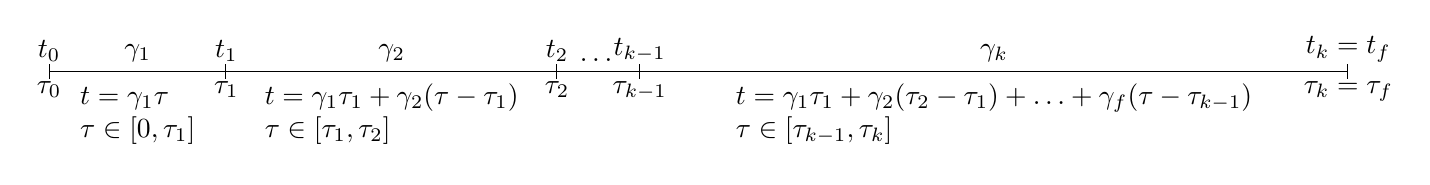
\begin{tikzpicture}[scale=1.5, domain=0:4, samples=200]
	    \draw [|-|](0,0) node[above] {$t_0$} node[below] {$\tau_0$} -- (1.5,0) node[midway, above] {$\gamma_1$} node[midway, below] {\begin{tabular}{l}
	    	$t = \gamma_1\tau$ \\
	    	$\tau\in[0, \tau_1]$
	    	\end{tabular}};
	    \draw [-|](1.5,0) node[above] {$t_1$} node[below] {$\tau_1$} -- (4.3,0) node[midway, above] {$\gamma_2$} node[midway, below] {\begin{tabular}{l}
	    	$t = \gamma_1\tau_1+\gamma_2(\tau-\tau_1)$ \\
	    	$\tau\in[\tau_1, \tau_2]$
	    	\end{tabular}};
	    \draw [-|](4.3,0) node[above] {$t_2$} node[below] {$\tau_2$} -- (5,0) node[midway,above] {\dots};
	    \draw [-|](5,0) node[above] {$t_{k-1}$} node[below] {$\tau_{k-1}$} -- (11,0) node[midway, above] {$\gamma_k$} node[midway, below] {\begin{tabular}{l}
	    	$t = \gamma_1\tau_1+\gamma_2(\tau_2-\tau_1)+\dots+\gamma_f(\tau-\tau_{k-1})$ \\
	    	$\tau\in[\tau_{k-1}, \tau_k]$
	    	\end{tabular}} node[above] {$t_k = t_f$} node[below] {$\tau_k = \tau_f$};
	\end{tikzpicture}
	\caption{Mehrere miteinander gekoppelte Zeitintervalle, die sich zu einem Gesamtintervall $[\tau_0, \tau_f]$ zusammensetzen.}
	\label{fig:Zeittransformation}
\end{figure}
Für die einzelnen Teilintervalle gelten dabei die dargestellten Zeittransformationen, sodass für das $j$-te Teilintervall
\begin{equation}
	\frac{\partial t}{\partial\tau} = \gamma_j \,, \quad\textrm{mit}\, j=1,2,...,k
\end{equation}
und damit 
\begin{equation}
\ve{z}_j'(\tau) = 
\gamma_j
\begin{bmatrix}
\ve{f}(\xoftau,\uoftau,\tau) \\
-\frac{\partial H}{\partial \ve{x}}
\end{bmatrix} 
\end{equation} 
gilt. Auch hier lassen sich die festen Intervallgrenzen ohne Einschränkung der Allgemeinheit zu
\begin{equation}
	\tau_0 = 0\,, \quad\tau_j = j\,, \quad\textrm{mit}\, j=1,2,...,k
\end{equation}
wählen, sodass für die freien Intervallgrenzen 
\begin{align}
t_0 &= \tau_0 \\
t_1 &= \gamma_1 \\
t_2 &= \gamma_1+\gamma_2 \\
&\vdots\\
t_f = t_k &= \gamma_1+\gamma_2+\dots+\gamma_k
\end{align}
gilt. Mithilfe dieser Erweiterung lassen sich beliebig viele Intervalle fester Intervallgrenzen auf Intervalle freier Grenzen transformieren. Eine Anwendung derartig verknüpfter Zeittransformationen kann nützlich sein, wenn mehrere Optimierungsprobleme, die jeweils für ein Teilintervall gelten, betrachtet werden und die Übergangsstellen $t_j$ frei und damit Teil der Optimierung sein sollen. Dann lassen sich die entsprechenden Teilintervalle mit festen Grenzen definieren und wie dargestellt mithilfe der Transformationsvorschriften auf die gesuchten, freien Intervallgrenzen abbilden.
\section{Variationsprobleme mit internen Gleichungsnebenbedingungen}\label{sec:InterneGNB}
Es kann durchaus von Interesse sein, neben den \gls{RB} an den Zeitpunkten $t_0$ und $t_f$ zusätzliche interne \gls{RB} der Form
\begin{equation}
	\tilde{\ve{g}}(\xoftone,t_1) = 0
\end{equation} zu formulieren, die die optimalen Trajektorien erfüllen sollen, wenn das dynamische System beispielsweise einen bestimmten Zustand zu einem gewissen Zeitpunkt $t_1$ erreichen soll \cite{Papageorgiou.2012}. Dazu wird auch in diesem Fall das Gütefunktional in Gleichung \ref{eq:J_var_sys} analog zur Betrachtung allgemeiner Endbedingungen erweitert. Allgemein können die Systemzustände und die adjungierten Zustände an der Stelle $t_1$ unstetig sein, weshalb es zweckmäßig ist, die Zeitpunkte $t_1^-$ und $t_1^+$ als die Zeitpunkte unmittelbar vor und nach der Sprungstelle $t_1$ zu definieren. Das erweiterte Gütefunktional lautet
\begin{equation}
\begin{split}
J(\ve{x},\dx,\ve{u},t,t_f,t_1) &= \underbrace{\Vofxoftf + \ve{\nu}^T\ve{g}(\xoftf,t_f) + \Vofxoftone + \tilde{\ve{\nu}}^T\tilde{\ve{g}}(\xoftoneminus,\xoftoneplus,t_1)}_{\Vofxoftoftonefallgemein} + \dots \\
\dots&+\int_{t_0}^{t_f}l(\ve{x},\ve{u},t) + \ve{\lambda}^T(\ve{f}(\ve{x},\ve{u},t) - \dx)\dtint{t}\,. \label{eq:J_var_sys_t1}
\end{split}
\end{equation}
und man erhält die Transversalitätsbedingungen \cite{Gerdts.2010}
\begin{align}
\Big(\frac{\partial \tilde{V}}{\partial \xoftoneminus} + (\frac{\partial \tilde{\ve{g}}}{\partial \xoftoneminus})^T\tilde{\ve{\nu}} - \lambdaoftoneminus\Big) &= 0 \label{eq:Sprungbedingung1}\\
\Big(\frac{\partial \tilde{V}}{\partial \xoftoneplus} + (\frac{\partial \tilde{\ve{g}}}{\partial \xoftoneplus})^T\tilde{\ve{\nu}} + \lambdaoftoneplus\Big) &= 0 \label{eq:Sprungbedingung1}\\
H(\ve{x},\ve{u},\ve{\lambda},t)_{|t=t_1^-} - H(\ve{x},\ve{u},\ve{\lambda},t)_{|t=t_1^+} + \Big(\frac{\partial \tilde{V}}{\partial t}+(\frac{\partial \tilde{\ve{g}}}{\partial t})^T\tilde{\ve{\nu}}\Big)_{|t=t_1}&= 0\,,\quad \textrm{falls, $t_1$ frei ist.}\label{eq:Transversalität_t1}
\end{align}

\textbf{Gleichungen überprüfen und weierstaß erdmann bedingunen erklären, literaturVZ updaten}
\section{Numerische Lösungsverfahren}\label{sec:Lösungsverfahren}
An dieser Stelle zeigt sich bereits ein wesentlicher Unterschied in der Lösbarkeit zwischen statischen und dynamischen Optimierungsproblemen. Bei statischen Optimierungsproblemen bedeuten zusätzliche Optimierungsvariablen lediglich ein größer dimensioniertes Problem und dadurch mehr Rechenaufwand, während die Lösbarkeit dadurch unbeeinflusst bleibt (vorausgesetzt die zusätzlichen Variablen und Gleichungen sind sinnvoll formuliert). Bei dynamischen Optimierungsproblemen hingegen bedeutet jede Änderung der Optimierungsvariablen oder des Gütefunktionals geänderte Zusammenhänge für die kanonischen \gls{DGL}. Dies kann leicht dazu führen, dass sich keine Lösung für die \gls{DGL} mehr finden lässt. 